\chapter*{Executive Summary}

Data and information systems play a critical role in environmental compliance management due to the large number of data types collected and sizable quantities of data that must be stored.  This data must be efficiently managed and processed into actionable information to track compliance with current regulatory policy and guide future development in response to changing environmental factors.

A gap analysis was conducted on the Environmental Information Systems (EISs) used by the Kuwait Environment Public Authority (KEPA) to determine if current capabilities are adequate to meet responsibilities defined under the Environment Protection Law 42/2014 (EPL); and if not, identify opportunities for improvement.  The gap analysis was conducted by a consultant under the United Nations Development Program (UNDP) Kuwait Environmental Governance Initiative (KEGI).

KEPA has invested heavily in advanced EISs and methods to enhance implementation of their regulatory programs. Nonetheless, the project found that KEPA has significant gaps in data management, compliance applications and training.  These gaps serve as opportunities for improving the existing EIS and capabilities and will ensure that KEPA can efficiently meet their compliance obligations under the EPL, as well as assist in meeting their long term Sustainable Development Goals (SDGs).  In addition to data gaps, findings also indicate redundancy in some EIS features as well as lack of interconnectivity between key EIS solutions.

While KEPA has many advanced EISs and very talented people operating them, the analysis identified several significant gaps in necessary data management applications required to effectively administer the by-laws and regulations of the EPL, as well as deficiencies in data processing methods relative to accepted management practices. Major findings include:

\begin{itemize}

\item Storing raw data in local spreadsheets without supporting metadata and providing summary statistics to the central eMISK data center for manual review and uploading.
\item No formal environmental incident reporting system to report spills, flares, or unplanned releases. Current notification is done via WhatsApp and instant messaging applications. 
\item No compliance management system that tracks authorized permits, certificates, and violation history for stakeholders. Current violation system only tracks violations assigned to an individual, not businesses or facilities.
\item Metadata was not collected for critical parameters.
\item Lack of familiarity among staff of common statistical analysis software packages and KEPA EISs. 
\item Standardized reporting formats and methods not issued to stakeholders.
\end{itemize}

Many of the findings can be simply resolved by reporting data using Electronic Data Deliverables (EDDs) through the Environmental Quality Information System (EQuIS) installed under the Compliance Information Management System (CIMS) project. EQuIS allows departments to submit raw data, review it for errors, store the technically correct data in a central server, and allow eMISK to access the raw data to calculate consistent summary statistics to populate their domains, instead of relying on departments to provide statistics. The EQuIS should be expanded to handle raw data, both data generated by KEPA and by external stakeholders, and integrated into the eMISK data processing methodology.

Other recommendations include:

\begin{itemize}
\item Adopt an international industrial code such as the UN's International Standard Industrial Code (ISIC) to classify individual stakeholder facilities.
\item Issue a KEPA policy on how to handle missing data, censored measurements (measurements below the level of detection of the instrument), and outliers.
\item Implement incident and compliance management software.
\item Issue nation-wide laboratory analysis and reporting methodologies for common analytical tests.
\item Publish official English translations of promulgated by-laws and regulations.

\end{itemize}

\clearpage

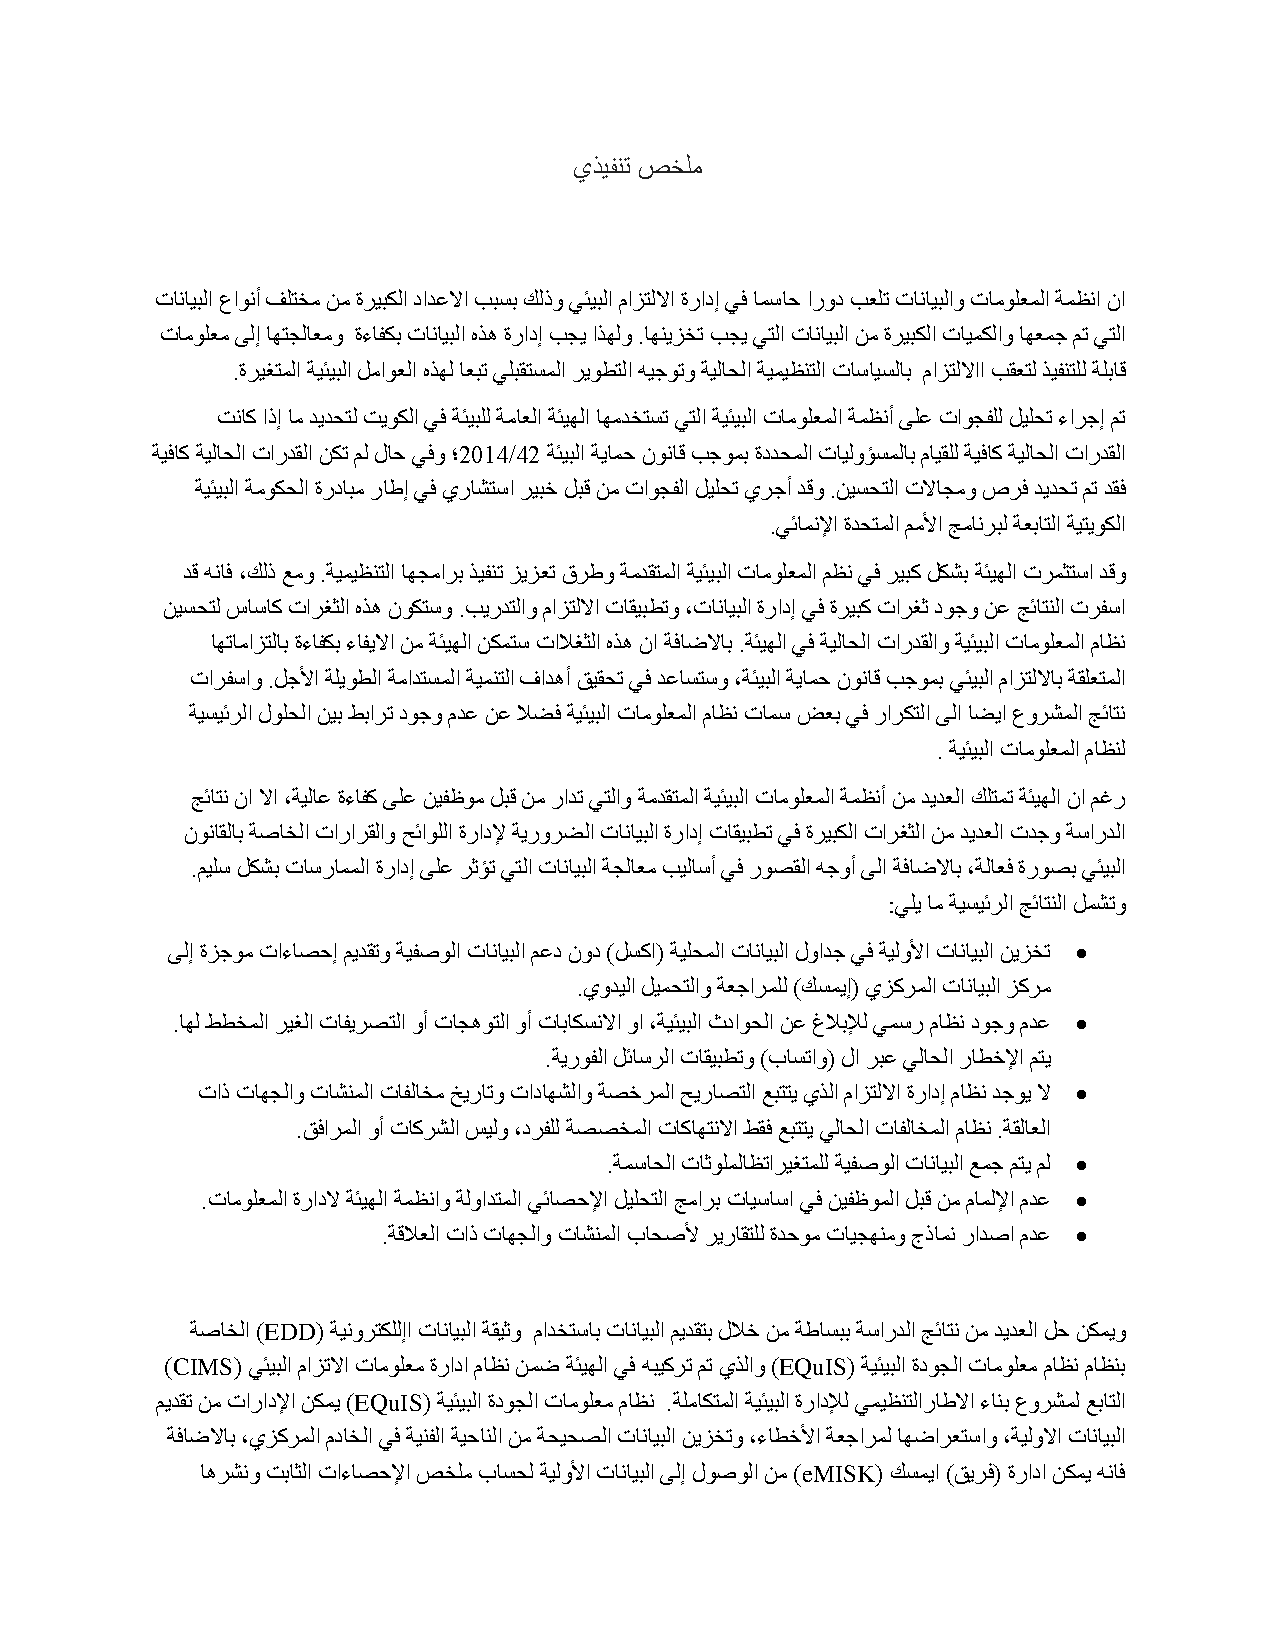
\includepdf[pages=-]{ExecutiveSummary-translatedAR.pdf}
